Ein weiterer Sensor, welcher für die Bodentemperaturmessung verwendet wird,
sind Thermoelemente. Grundlage dieses Sensors ist eine Verbindung zweier Drähte
unterschiedlicher Materialien.Die Funktionsweise des Sensors basiert auf
thermoelektrischen Effekten. Der sogenannte Peltier-Effekt besagt hierbei, dass
bei einer Verbindung von zwei, unter Strom stehenden Drähten aus
unterschiedlichen Materialien ein Wärmestrom fließt. Dieser wird an der
Verbindungsstelle absorbiert, was dort zu einer Temperaturveränderung des
Materials führt. Der Seebeck-Effekt geht auf den Stromfluss bei einer
Temperaturänderung ein. Bei der Verbindung der zwei Leiter kommt es zu einem
Stromfluss, wenn an beiden Verbindungsstellen unterschiedliche Temperaturen
anliegen. \cite{bernhard2014thermoelemente}

\begin{figure}[ht]
	\centering
	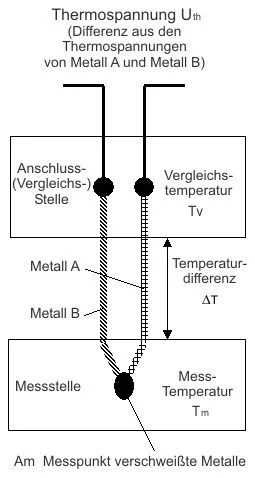
\includegraphics[width=0.5\textwidth]{bilder/thermoelement.jpg}
	\caption[Aufbau Thermoelement]{Aufbau eines Thermoelements}
	\label{fig:thermoelement}
\end{figure}

